% Generated from upstream slc-screen.tex at 6178f32f61645f3b62ef621b4c5a88f8e67778ad.
% Localized settings are loaded from the accompanying preamble files.
% slc-screen.tex

% driver file slc-screen.tex to produce the Sets, Logic, Computation
% textbook on with same type block as in printed version, but but with
% on-screen features (color, links, etc).

\input{olpkit-before-class}
\documentclass[screen]{../../../../sty/open-logic-book}

\usepackage[all]{nowidow}
\input{locale/mr/config/slc-fonts}

\definecolor{OLPcolor}{RGB}{248,154,14}
\definecolor{OLPdkcolor}{RGB}{104,65,6}
\definecolor{OLPltcolor}{RGB}{248,203,137}

\def\oljobname{slc}
\newcommand{\olpath}{../../../..}
\input{olpkit-before-olp}
\input{\olpath/sty/open-logic.sty}
\input{olpkit-after-olp}

\begin{document}
\raggedbottom

\OLPscreencover{%
  \hfill\hspace{.29\textwidth}\includegraphics[width=.29\textwidth]{\olpath/assets/portraits/cantor-circle.pdf}\hfill{}

  \hfill{}
  \includegraphics[width=.29\textwidth]{\olpath/assets/portraits/goedel-circle.pdf}
  \hfil\includegraphics[width=.29\textwidth]{\olpath/assets/portraits/turing-circle.pdf}\hfil{}
  \includegraphics[width=.29\textwidth]{\olpath/assets/portraits/skolem-circle.pdf}
  \hfill{}

  \hfill{}
  \includegraphics[width=.29\textwidth]{\olpath/assets/portraits/noether-circle.pdf}\hspace{.29\textwidth}\hfill{}
}

% Now load the actual text

% Generated from upstream slc.tex at 6178f32f61645f3b62ef621b4c5a88f8e67778ad.
% Localized settings are loaded from the accompanying preamble files.
% slc.tex
%
% driver file slc.tex to produce text

\newif\ifslcChapterSummaries
\slcChapterSummariestrue
\preto\OLEndChapterHook{%
  \ifslcChapterSummaries
  \edef\slcSummaryFile{include/summary-\number\value{chapter}.tex}%
  \IfFileExists{\slcSummaryFile}{%
    \section*{सारांश}\addcontentsline{toc}{section}{सारांश}%
    {\let\emph\textbf\input{\slcSummaryFile}}}{}%
  \fi
}

\problemsperchapter

\frontmatter

\OLPfrontmatter

\cleartoverso
\thispagestyle{empty}
\ \vfill
\noindent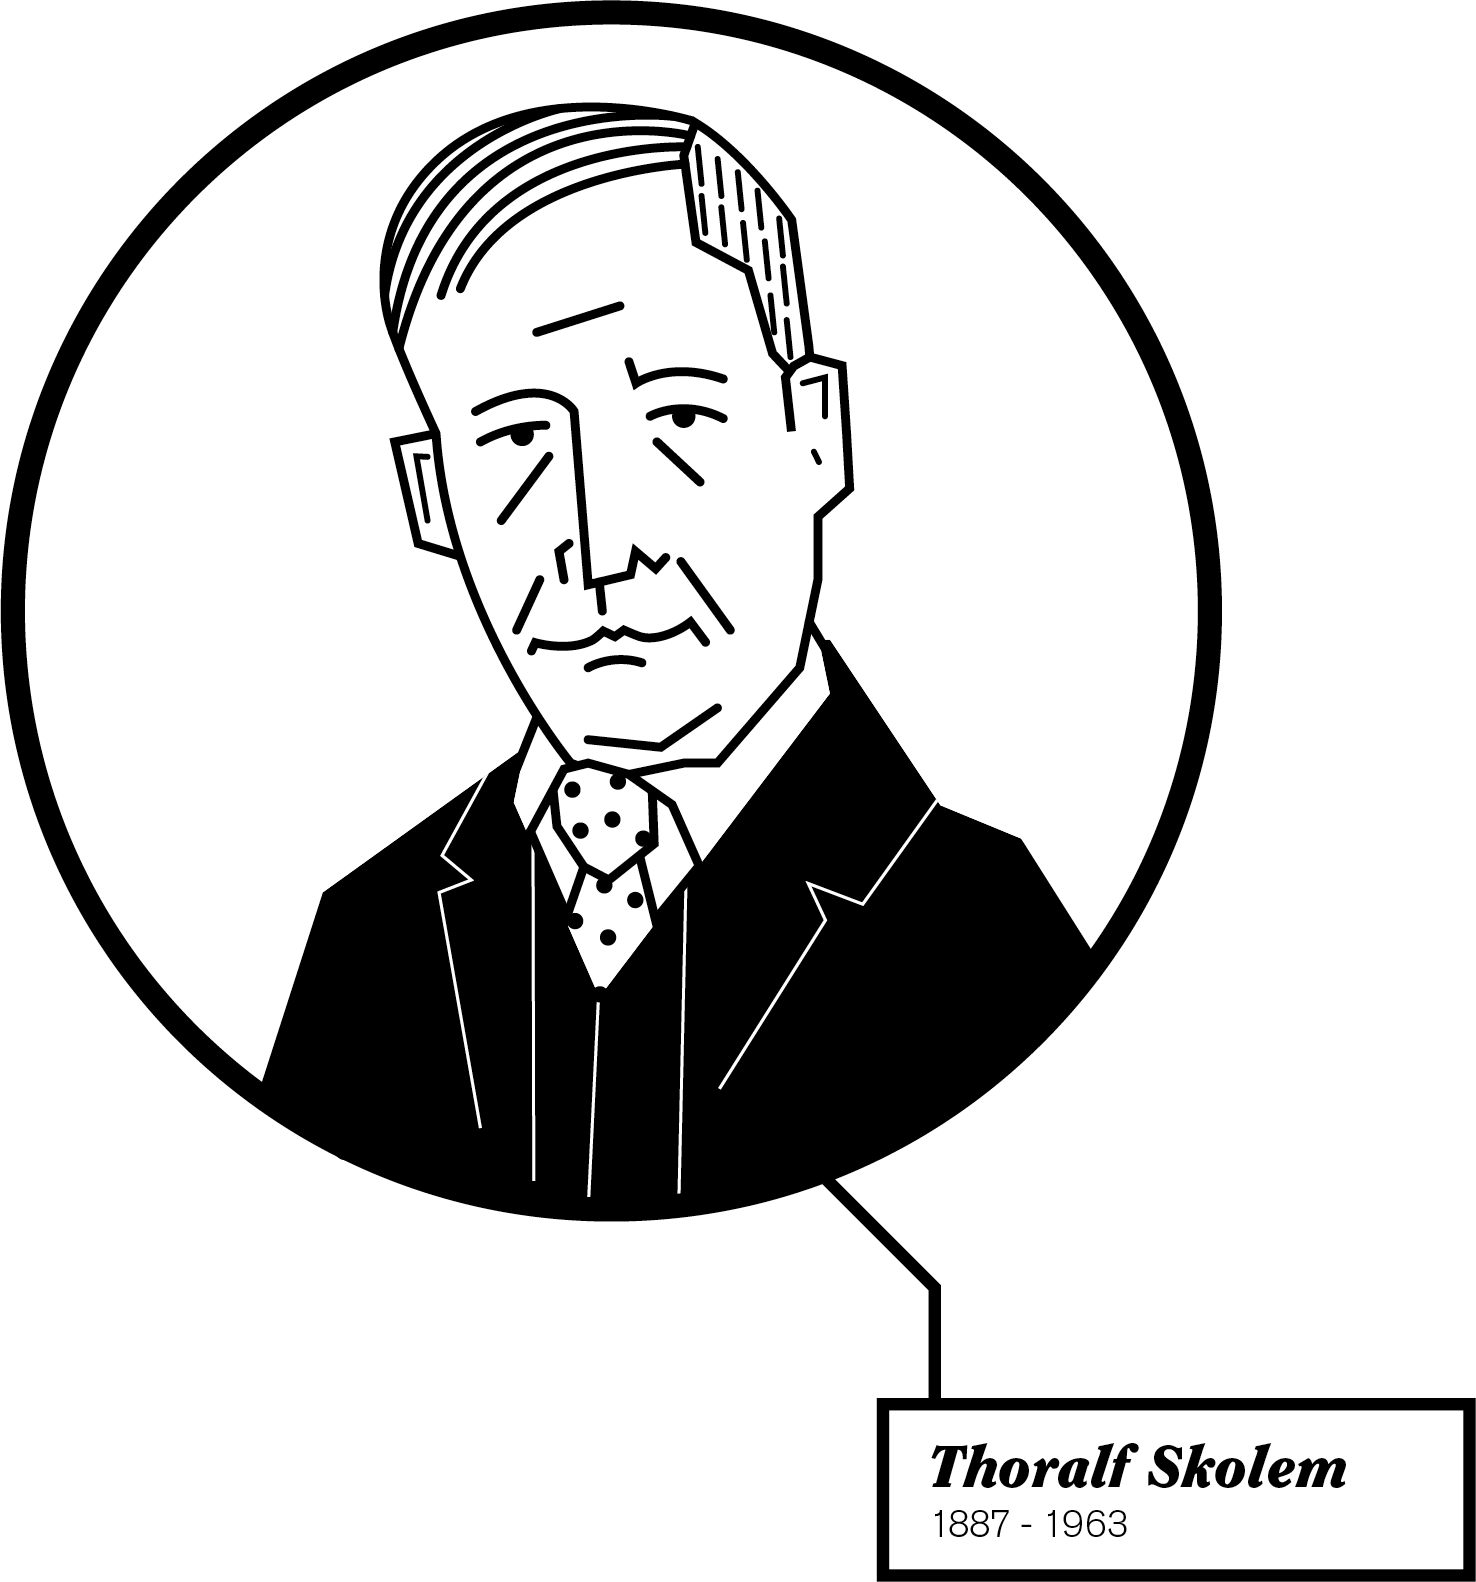
\includegraphics[width=\textwidth]{illustrations/SkolemChapter}
\vfill

\chapter{प्रस्तावना}

हे पुस्तक अधितर्कशास्त्राचा परिचय करून देते. ते विशेषतः संगणकशास्त्र आणि तत्त्वज्ञान यांच्या विद्यार्थ्यांसाठी आहे. तर्कशास्त्राचाच अभ्यास करणारी शाखा असल्यामुळे तिला ``अधितर्कशास्त्र'' असे नाव आहे. तर्कशास्त्रात वैध अनुमानाच्या नियमांचा विचार केला जातो. तर्कशास्त्राचे चिन्हात्मक किंवा आकारिक रूप हे नियम विधानीय किंवा प्रथम-क्रम तर्कशास्त्राच्या भाषांसारख्या आकारिक भाषांत मांडते. अधितर्कशास्त्रात या भाषांचे आणि त्या वापरून केलेल्या योग्य अनुमानाच्या नियमांचे गुणधर्म तपासले जातात. या आकारिक भाषांतील अभिव्यक्तींना नेमका अर्थ कसा द्यावा, वैध अनुमानाच्या नियमांचे समर्थन कसे करावे आणि विविध !!{derivation} पद्धतींचे गुणधर्म, त्यांच्या संगणनविषयक गुणधर्मांसह, कोणते आहेत, अशा प्रश्नांचा त्यात विचार होतो. येथे तपासलेल्या भाषा आणि !!{derivation} पद्धती अनेक क्षेत्रांत, विशेषतः गणित, तत्त्वज्ञान, संगणकशास्त्र आणि भाषाविज्ञान यांत वापरल्या जातात. त्यामुळे हे प्रश्न स्वतःच महत्त्वाचे आणि रंजक आहेत. शिवाय, सर्वसाधारणपणे आकारिक प्रणाल्यांचा अभ्यास कसा करावा हेही त्यांतून दिसते. येथे आपण ज्या तार्किक भाषा अभ्यासतो त्यांखेरीज इतरही भाषा अभ्यासकांच्या दृष्टीने महत्त्वाच्या आहेत. उदाहरणार्थ, भाषावैज्ञानिक आणि तत्त्वज्ञ यांना विधानीय व प्रथम-क्रम तर्कशास्त्राच्या भाषांपेक्षा कितीतरी गुंतागुंतीच्या भाषांत रस असतो. संगणकशास्त्रज्ञांना तर प्रोग्रामिंग भाषांसारख्या वेगळ्याच \emph{प्रकारच्या} भाषांत रस असतो. आकारिक भाषांची चिन्हार्थमीमांसा कशी द्यावी, त्यांच्याविषयीचे निष्कर्ष कसे सिद्ध करावेत आणि त्यांचे गुणधर्म कसे तपासावेत, यासाठी आपण पाहणार असलेल्या पद्धती तिथेही लागू होतात.

इतर कोणत्याही विद्याशाखेप्रमाणे अधितर्कशास्त्रातही निष्कर्ष किंवा तथ्ये आहेत आणि पद्धती व तंत्रेही आहेत. या पुस्तकात दोन्हींचा विचार केला आहे. पुष्कळ विद्यार्थ्यांना हा अभ्यासक्रम संपल्यावर आपण पाहिलेल्या प्रत्येक निष्कर्षाची गरज पडणार नाही, पण ते निष्कर्ष प्रस्थापित करण्यासाठी आपण ज्या पद्धती वापरतो त्यांची त्यांना गरज पडेल आणि ते त्या वापरतील. उदाहरणार्थ, लोव्हेनहाइम--स्कोलेम प्रमेय संगणकशास्त्रात वारंवार वापरले जात नाही, पण त्याच्या सिद्धतेसाठी आपण वापरतो त्या पद्धती तिथे वापरल्या जातात. याउलट, आपण पाहणार असलेले अनेक निष्कर्ष विज्ञानाचे तत्त्वज्ञान आणि सत्तामीमांसा यांतील काही वादांना लागू पडतात. तत्त्वज्ञानाच्या विद्यार्थ्यांना अभ्यासक्रमाबाहेर हे निष्कर्ष सिद्ध करता येण्याची गरज भासेलच असे नाही, पण त्यांचा आशय समजला पाहिजे. ते प्रस्थापित करण्यासाठी लागणाऱ्या व्याख्यांचा आणि सिद्धतांचा नीट विचार केला तरच हे निष्कर्ष खऱ्या अर्थाने \emph{समजतात}. या पुस्तकातील निष्कर्ष आणि पद्धती यांचा अभ्यास संगणकशास्त्र व तत्त्वज्ञान यांच्या विद्यार्थ्यांना सुचवला जातो, आणि काही अभ्यासक्रमांत तो आवश्यकही असतो, याची ही काही कारणे आहेत.

पुस्तकाचे तीन भाग आहेत. \Olref[sfr][][]{part} संचसिद्धान्ताविषयी आहे. तर्कशास्त्र व अधितर्कशास्त्र यांचा ``गणिताची पायाभरणी'' असे ज्याला म्हणतात त्याच्याशी ऐतिहासिकदृष्ट्या निकटचा संबंध आहे. पूर्णांक, परिमेय व वास्तव संख्या, फलने, अवकाश इत्यादी गणितीय वस्तू मुळात कशा समजून घ्याव्यात हा त्या अभ्यासाचा विषय आहे. संचसिद्धान्त त्याचे एक उत्तर देतो (इतरही उत्तरे आहेत). म्हणूनच संचसिद्धान्त आणि तर्कशास्त्र यांचा दीर्घकाळ एकत्र अभ्यास होत आला आहे. कोणत्याही प्रकारच्या आकारिक अभ्यासात संच, संबंध आणि फलने सर्वत्र आढळतात. गणिताबरोबरच संगणकशास्त्रात आणि तत्त्वज्ञानाच्या काही अधिक तांत्रिक शाखांतही ती दिसतात. तर्कशास्त्राची चिन्हार्थमीमांसा, सिद्धता उपपत्ती आणि संगणनक्षमतेची पायाभूत तत्त्वे यांविषयी निष्कर्ष मांडण्यासाठी व सिद्ध करण्यासाठी योग्य परिभाषा असणे आवश्यक आहे. उदाहरणार्थ, आपण अभिव्यक्तींचे संच, तार्किक निष्पन्नतेचे व सिद्धतायोग्यतेचे संबंध, विधेयचिन्हांचे अर्थनिर्धारण (त्यातून संबंधच मिळतात), संगणनक्षम फलने, त्यांच्यातील विविध संबंध आणि त्यांचा वापर करून केलेल्या विविध रचना यांविषयी बोलू. यासाठी संक्षिप्त संकेत असणे आणि संच, संबंध व फलने यांच्या सर्वसाधारण गुणधर्मांचा विचार करणे सोयीचे ठरेल. गणितीय विचार करण्याची आणि गणितीय सिद्धता मांडण्याची सवय नसेल, तर संचसिद्धान्ताचा पहिला भाग सरावाची संधी समजा. सर्व मूलभूत व्याख्या दिल्या जातील आणि त्यांचा वापर करून क्रमाक्रमाने अधिक गुंतागुंतीच्या सिद्धता दिल्या जातील. विशेषतः पहिल्या भागात, या सिद्धता समजून घेणे आणि त्या स्वतः शोधून मांडता येणे हे बहुधा निष्कर्ष समजून घेण्यापेक्षा अधिक महत्त्वाचे आहे. गणितीय विचार करण्याची तुम्हाला सवय नसेल, तर उदाहरणांचा आणि समस्यांचा नीट विचार करणे महत्त्वाचे आहे.

पहिल्या भागात मात्र आपण एक महत्त्वाचा निष्कर्ष प्रस्थापित करू. हा निष्कर्ष म्हणजे कँटरचे प्रमेय. विज्ञानात संकल्पनाविश्लेषणाची जी अत्यंत उल्लेखनीय उदाहरणे आढळतात त्यांपैकी एका उदाहरणावर तो आधारलेला आहे. ते म्हणजे कँटर यांनी केलेले अनंततेचे विश्लेषण. अनेक शतके गणितज्ञ आणि तत्त्वज्ञ दोघांनाही अनंततेने कोड्यात टाकले आहे. कँटर यांच्यापूर्वी तिचा नेमका विचार कसा करावा हे कोणालाच ठाऊक नव्हते. तिचा विचार करणे हीच चूक आहे आणि अनंत संग्रह ही कल्पनाच विसंगत आहे असेही पुष्कळांना वाटत असे. कँटर यांनी अनंततेचा सुसंगतपणे अभ्यास करणे शक्य केले. त्यांनी अनंत संग्रहांची आणि त्या संग्रहांचे आकारमान मोजता येईल अशा अनंत संख्यांची संपूर्ण उपपत्ती विकसित केली. अनंततेच्या वेगवेगळ्या पातळ्या आहेत हे त्यांनी दाखवले. ``अनंतपार'' संख्यांची ही उपपत्ती सुंदर आणि गुंतागुंतीची आहे. आपण तिच्यात फार खोलवर जाणार नाही, पण अनंततेच्या वेगवेगळ्या पातळ्या आहेत, विशेषतः ``गणनीय'' आणि ``अगणनीय'' पातळ्या आहेत, हे दाखवू शकू. या निष्कर्षाचे महत्त्वाचे उपयोग आहेत. शिवाय आपल्या विषयाची जाण ठेवू इच्छिणाऱ्या प्रत्येक गणितज्ञाला, संगणकशास्त्रज्ञाला आणि तत्त्वज्ञाला माहीत असावा असा हा निष्कर्ष आहे.

\olref[fol][][]{part} मध्ये आपण प्रथम-क्रम तर्कशास्त्राकडे वळतो. आपण प्रथम-क्रम तर्कशास्त्राची भाषा आणि तिची चिन्हार्थमीमांसा यांची व्याख्या करू. म्हणजेच प्रथम-क्रम रचना म्हणजे काय आणि प्रथम-क्रम तर्कशास्त्राचे वाक्य एखाद्या रचनेत केव्हा सत्य ठरते हे ठरवू. यामुळे आपल्याला दोन महत्त्वाच्या गोष्टी करता येतील. (1)~एखादे वाक्य दुसऱ्या वाक्यापासून तार्किकरीत्या केव्हा निष्पन्न होते हे गणितीय काटेकोरपणे सांगता येईल. (2)~प्रथम-क्रम रचनेतील संबंधांचे वर्णन, म्हणजेच त्यांचे लक्षणचित्रण, त्या रचनांमध्ये सत्य असणारी वाक्ये कशा रीतीने करतात हे पाहता येईल. यातून विशेषतः स्वयंसिद्धकीय पद्धतीची चर्चा पुढे येते. या पद्धतीत विशिष्ट प्रकारच्या रचनांचे लक्षणचित्रण करण्यासाठी प्रथम-क्रम भाषांतील वाक्ये वापरली जातात. पुढे आपण सिद्धता उपपत्ती पाहू. त्यात गरहार्ड गेंटझेन यांनी १९३० च्या दशकात परिभाषित केलेली क्रमवर्ती कलनाची आणि नैसर्गिक निगमनाची मूळ रूपे पाहू. (तुमचे अध्यापक यांपैकी एकच पद्धत शिकवण्याचे ठरवू शकतात. तसे झाल्यास ``!!{derivation}s'' आणि ``!!{derivability}'' यांचा उल्लेख त्यांनी निवडलेल्या पद्धतीच्या संदर्भात समजावा.) एखादे वाक्य इतर काही वाक्यांवरून निष्पन्न होते ही कल्पना नेमकी करण्याचे दोन सर्वस्वी वेगळे मार्ग आपल्याला मिळतात. एक म्हणजे तार्किक निष्पन्नतेची चिन्हार्थविषयक संकल्पना आणि दुसरा म्हणजे !!{derivability} ची विन्यासात्मक संकल्पना. निर्दोषता आणि संपूर्णता ही प्रमेये या दोन लक्षणचित्रणांचा संबंध जोडतात. विशेषतः आपण गोडेल यांचे संपूर्णता प्रमेय सिद्ध करू. त्यानुसार एखादे वाक्य इतर काही वाक्यांपासून चिन्हार्थाच्या दृष्टीने निष्पन्न होत असेल, तर ते त्यांच्यापासून !!{derivable} ही असते. याची समतुल्य मांडणी अशी आहे. एखादा वाक्यसंच सुसंगत असेल, म्हणजे त्यावरून व्याघात सिद्ध करता येत नसेल, तर ती सर्व वाक्ये सत्य ठरतील अशी एखादी रचना असते.

संपूर्णता प्रमेयाची दुसरी मांडणी कदाचित अधिक आश्चर्यकारक आहे. गोडेल यांनी हा निष्कर्ष सिद्ध केला त्या सुमारास (१९२९ मध्ये) डाव्हीट हिल्बर्ट या जर्मन गणितज्ञाचे एक प्रसिद्ध मत असे होते की गणितीय अस्तित्वासाठी सुसंगतता, म्हणजे व्याघाताचा अभाव, एवढीच अट पुरेशी आहे. दुसऱ्या शब्दांत, एखाद्या रचनेचे किंवा रचनांच्या वर्गाचे सुसंगत वर्णन एखाद्या गणितज्ञाला करता येत असेल, तर अशा रचना अस्तित्वात आहेत असे मानण्याचा त्याला अधिकार असावा. त्या काळात अनेकांना ही कल्पना हास्यास्पद वाटली. एखाद्या रचनेचे वर्णन करताना आपण स्वतःशी विसंगत बोललो नाही, एवढ्यावरून ती रचना खरोखर अस्तित्वात आहे असा निष्कर्ष कसा निघणार? गोडेल यांचे संपूर्णता प्रमेय नेमके हेच सांगते. विरोधापत्तीसारख्या आणि तत्त्वज्ञानाच्या दृष्टीने कुतूहलजनक अशा या पैलूबरोबरच संपूर्णता प्रमेयाचे दोन महत्त्वाचे उपयोगही आहेत. दिलेली वाक्ये सत्य ठरवणाऱ्या रचनांच्या अस्तित्वाविषयी आणखी निष्कर्ष सिद्ध करण्यासाठी ते उपयोगी पडतात. हे निष्कर्ष म्हणजे संहतता प्रमेय आणि लोव्हेनहाइम--स्कोलेम प्रमेय.

\olref[tur][][]{part} मध्ये आपण तर्कशास्त्राचा संबंध संगणनक्षमतेशी जोडतो. यालाही ऐतिहासिक संदर्भ आहे. तर्कशास्त्रातील एखादे दिलेले वाक्य सिद्ध करता येते की नाही हे ठरवणारी यांत्रिक पद्धत शोधणे ही तर्कशास्त्राची एक मूलभूत समस्या म्हणून डाव्हीट हिल्बर्ट यांनी मांडली होती. विधानीय तर्कशास्त्रासाठी अशी पद्धत अर्थातच आहे. सर्व सत्यताकोष्टके तपासली की झाले. ती सांत संख्येने असल्यामुळे या पद्धतीने अखेरीस योग्य उत्तर मिळते. प्रथम-क्रम तर्कशास्त्रासाठी इतकी सरळ पद्धत शक्य नाही, कारण संभाव्य रचना अनंत संख्येने असतात (आणि रचना स्वतःही अनंत असू शकतात). अधिक कल्पक पद्धत शोधण्यासाठी तर्कशास्त्रज्ञ अनेक वर्षे प्रयत्न करत होते. ॲलोन्झो चर्च आणि ॲलन ट्यूरिंग यांनी अखेरीस अशी कोणतीही पद्धत अस्तित्वात नसल्याचे सिद्ध केले. त्यासाठी सर्वसाधारणपणे यांत्रिक पद्धत म्हणजे काय याची प्रथम नेमकी व्याख्या देणे आवश्यक होते. एखादी निर्णयप्रक्रिया सुचवली गेली असती, तर बहुधा ती प्रभावी पद्धत आहे हे ओळखता आले असते. पण कोणतीही प्रभावी पद्धत अस्तित्वात नाही हे सिद्ध करण्यासाठी ``प्रभावी पद्धत'' याची आधी व्याख्या करावी लागते आणि त्या व्याख्येच्या आधारे अशक्यता सिद्ध करावी लागते. ट्यूरिंग यांनी हेच केले. तत्त्वतः एखाद्या यांत्रिक प्रक्रियेला काय करता येते याचे गणितीय प्रतिमान म्हणून त्यांनी ट्यूरिंग यंत्राची\footnote{अर्थात, ट्यूरिंग यांनी स्वतः त्याला हे नाव दिले नव्हते.} कल्पना मांडली. गणितीय साधनांनी एखाद्या अनौपचारिक संकल्पनेचे \emph{संकल्पनाविश्लेषण} करण्याचे हे आणखी एक उदाहरण आहे. कँटर यांचे अनंततेचे विश्लेषण गणिताला जितके महत्त्वाचे आहे, तितकेच हे विश्लेषण संगणकशास्त्राला कदाचित महत्त्वाचे आहे. शेवटचे मोठे काम म्हणजे अशक्यतेची दोन प्रमेये सिद्ध करणे. ``थांबण्याची समस्या'' म्हणून ओळखली जाणारी समस्या ट्यूरिंग यंत्रांना सोडवता येत नाही हे आपण दाखवू. शेवटी, तर्कशास्त्रासाठी हिल्बर्ट यांनी मांडलेली ``निर्णय समस्या''ही त्यांना सोडवता येत नाही हे दाखवू.

हे पुस्तक गणितीय आहे, कारण त्यात आपण गणितीय व्याख्यांची चर्चा करतो आणि आपले निष्कर्ष गणितीय रीतीने सिद्ध करतो. मात्र त्यासाठी गणिताचे विस्तृत पूर्वज्ञान आवश्यक नाही. पुस्तकातील कोणत्याही भागासाठी बीजगणित, त्रिकोणमिती किंवा कलन यांचे ज्ञान लागत नाही. गणितात काम कसे केले जाते याचाही आधीचा परिचय लागणार नाही याची आम्ही विशेष काळजी घेतली आहे. खरे तर, आपले निष्कर्ष समजून घेण्यासाठी आणि सिद्ध करण्यासाठी लागणारे युक्तिविचार आणि सिद्धता देण्याचे कौशल्य \emph{विकसित करणे} हा या पुस्तकाच्या हेतूचा एक भाग आहे. पुस्तकाची मांडणी गणितातील संकेतांनुसार आहे. गणितात स्पष्टता आणि काटेकोरपणा यांना विशेष महत्त्व असल्यामुळे हे संकेत विकसित झाले आहेत. उदाहरणार्थ, एखादी गोष्ट युक्तिवादाचा निष्कर्ष म्हणून मांडली आहे, दुसऱ्या गोष्टीच्या समर्थनार्थ दिली आहे की नव्या संज्ञेची ओळख करून देण्यासाठी आली आहे, हे समजणे आवश्यक असते. म्हणून आपण गणितातील संकेत पाळतो. नवीन संज्ञा किंवा चिन्हे देणाऱ्या मजकुराला ``व्याख्या'' असे म्हणतो आणि निष्कर्ष किंवा एखादी सिद्ध झालेली बाब नोंदवताना ``प्रमेय'', ``विधान'', ``पूर्वप्रमेय'' किंवा ``अनुप्रमेय'' असे म्हणतो. या संकेतांबरोबरच तर्कशास्त्राच्या पहिल्या अभ्यासक्रमातून कदाचित परिचित असलेल्या तार्किक सिद्धतेच्या पद्धती आपण वापरू. निष्कर्ष सिद्ध करण्यासाठी \emph{विगमन} पद्धतीचाही भरपूर वापर करू. परिशिष्टाची दोन प्रकरणे या सिद्धता-पद्धतींना वाहिलेली आहेत.

\paragraph{अध्यापकांसाठी सूचना} या पुस्तकातील सामग्री आकारिक तर्कशास्त्राच्या दुसऱ्या, एका सत्राच्या अभ्यासक्रमासाठी योग्य आहे. कॅलगरी विद्यापीठात मी तर्कशास्त्र~II या अभ्यासक्रमात ती १२ आठवड्यांत शिकवतो. मात्र पुस्तकात दिले आहे तितक्या तपशिलात सर्व विषय शिकवत नाही. उदाहरणार्थ, मी सामान्यतः फक्त नैसर्गिक निगमन शिकवतो आणि एकरूपतेसाठी संपूर्णतेच्या तपशीलवार सिद्धता वगळतो. विद्यार्थ्यांनी त्याआधी तर्कशास्त्र~I हा अभ्यासक्रम घेतलेला असतो. तो सहसा \emph{\href{https://forallx.openlogicproject.org}{forall x: Calgary}} या पुस्तकावरून शिकवला जातो. त्यात नैसर्गिक निगमनाचे हेच नियम वापरले आहेत, पण फिच यांच्या मांडणीत.

या पुस्तकाची सर्वांत अलीकडची PDF आवृत्ती \href{https://slc.openlogicproject.org}{मूळ पाठ्यपुस्तकाच्या संकेतस्थळावर} उपलब्ध आहे, पण ती वारंवार बदलते. CC BY परवान्यामुळे तुम्हाला स्वतः पुस्तक डाउनलोड करून वितरित करण्याचा अधिकार मिळतो.\footnote{CC BY 4.0 हा मजकुराचा परवाना आहे. या मराठी PDF मधील व्यक्तिचित्रे व छायाचित्रे वितरित करताना त्यांच्या स्वतंत्र वापराच्या अटी लागू होतात. त्या पुस्तकाच्या श्रेयपृष्ठांवर दिल्या आहेत.} तुम्ही ते वापरत असलेल्या संपूर्ण सत्रात सर्व विद्यार्थ्यांकडे एकच आवृत्ती असावी यासाठी या अधिकाराचा उपयोग करा. तुम्ही वापरायचे ठरवलेले PDF आपल्या शिक्षण व्यवस्थापन प्रणालीवर अपलोड करा. विद्यार्थ्यांना केवळ दुवा दिल्यास ते एकाच आवृत्तीचा वापर करतील याची खात्री राहत नाही. तुमच्या पुस्तकविक्रेत्याकडून तुम्ही PDF छापून घेऊ शकता. काही पुस्तकविक्रेत्यांना Amazon वर उपलब्ध असलेल्या मऊ मुखपृष्ठाच्या प्रती विकत घेऊन विक्रीसाठी ठेवता येतील.

ग्रॅहम लीच-क्राउस यांचे विनामूल्य ऑनलाइन तर्कशास्त्र अध्यापन साधन \emph{Carnap} (\href{https://carnap.io}{carnap.io}) प्रथम-क्रम तर्कशास्त्राची विन्यासमीमांसा, चिन्हार्थमीमांसा आणि सिद्धता-पद्धती यांच्या अभ्यासाला पूरक आहे. नैसर्गिक निगमन व क्रमवर्ती कलनातील !!{derivation}s, साध्या उपपत्तींसाठी रचना देणे आणि चिन्हांकन यांसारख्या सरावांची उत्तरे त्यात सादर करता येतात आणि त्यांचे स्वयंचलित मूल्यमापन होते. \href{https://turing.openlogicproject.org}{turing.openlogicproject.org} येथे ट्यूरिंग यंत्राचे अनुकरण करणारे साधनही आहे. \olref[tur][][]{part} मधील सामग्री उदाहरणांसह समजावण्यासाठी ते वापरता येते. तिथली उदाहरणे या साधनात आधीच भरलेली आहेत.


\cleartoverso 


\thispagestyle{empty}
\ \vfill
\noindent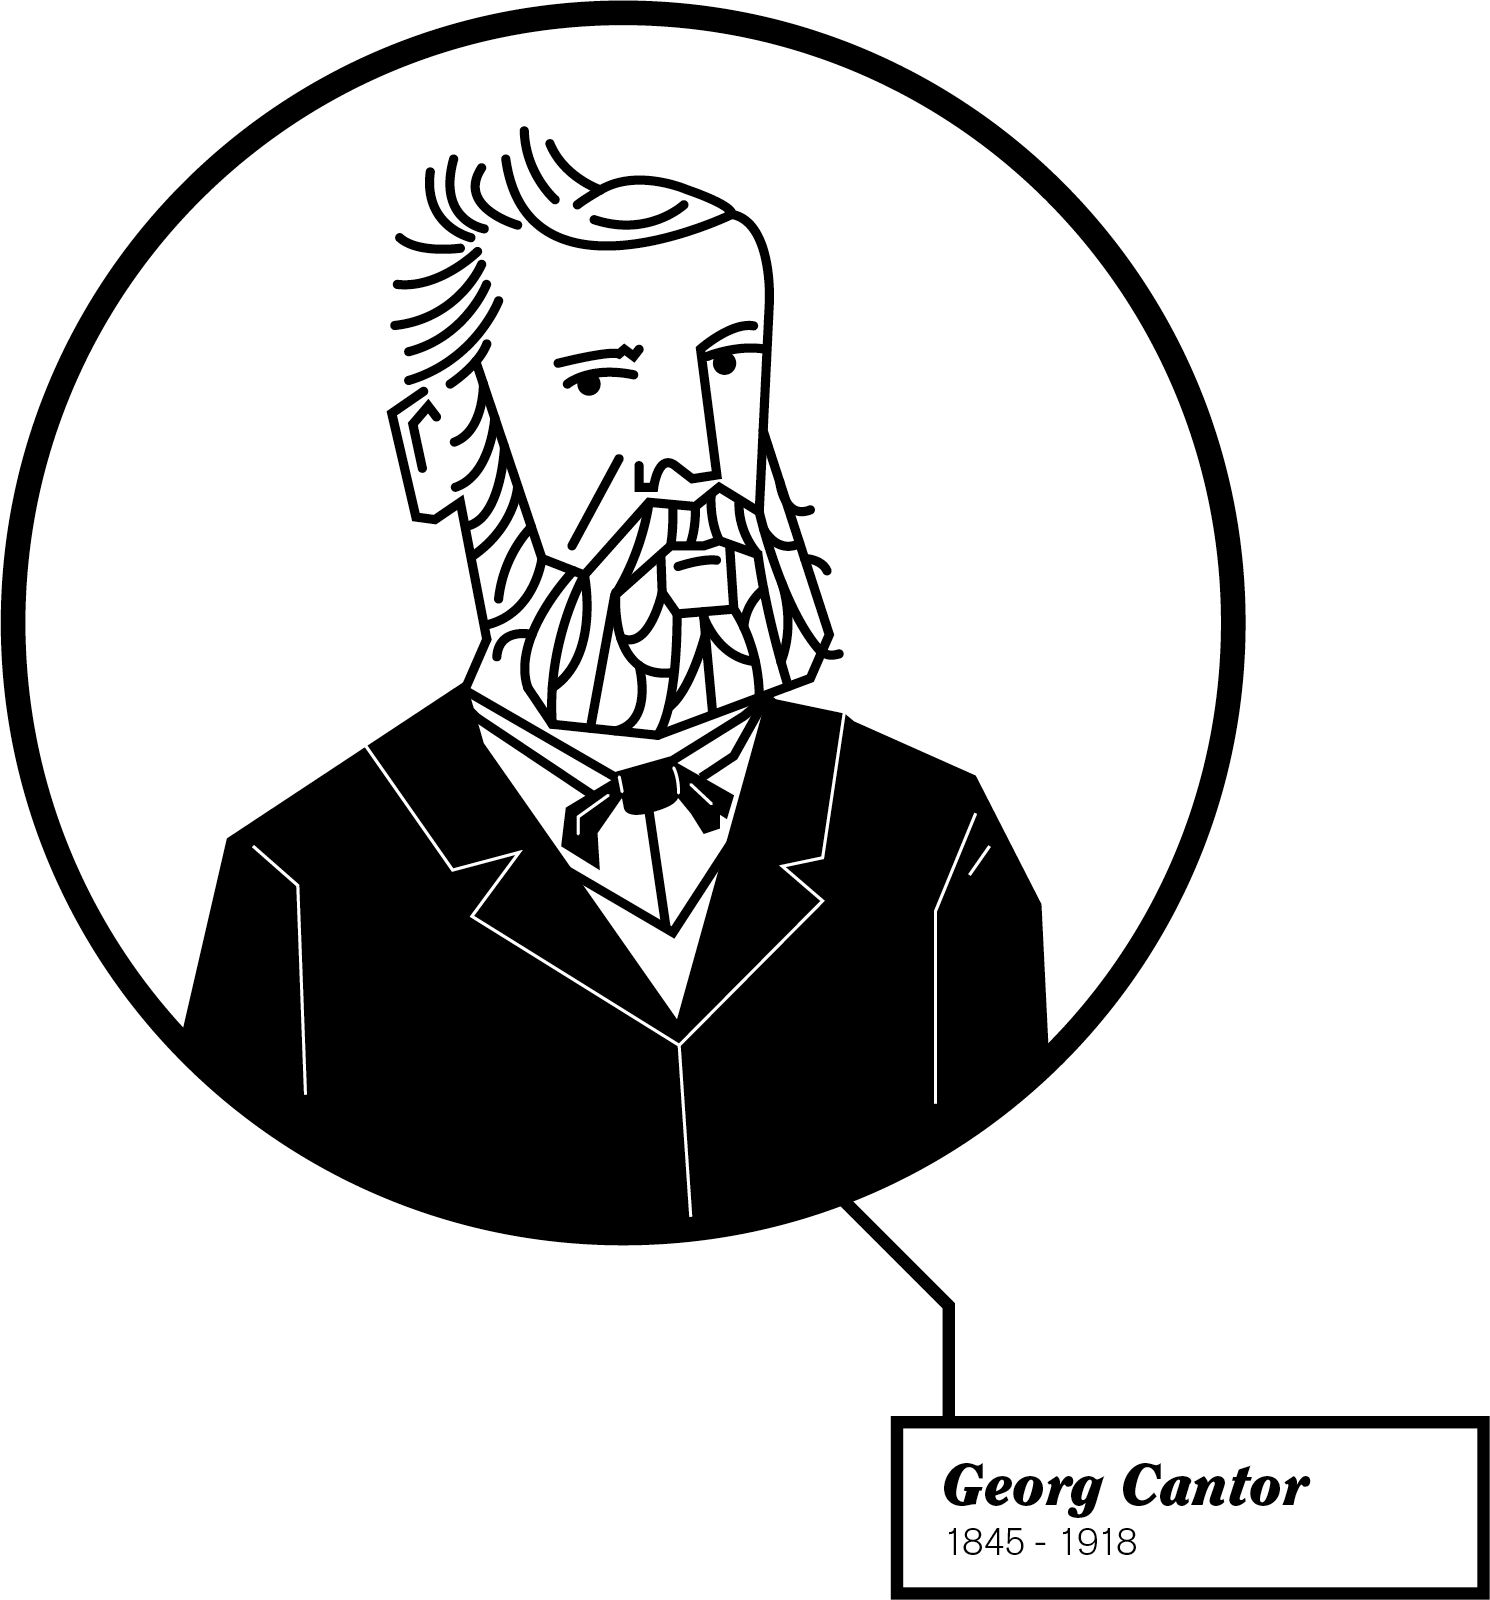
\includegraphics[width=\textwidth]{illustrations/CantorChapter}
\vfill

\mainmatter

\olimport*[sets-functions-relations]{sets-functions-relations}

\cleartoverso
\ifodd\value{page}\stepcounter{page}\fi
\thispagestyle{empty}
\ \vfill
\noindent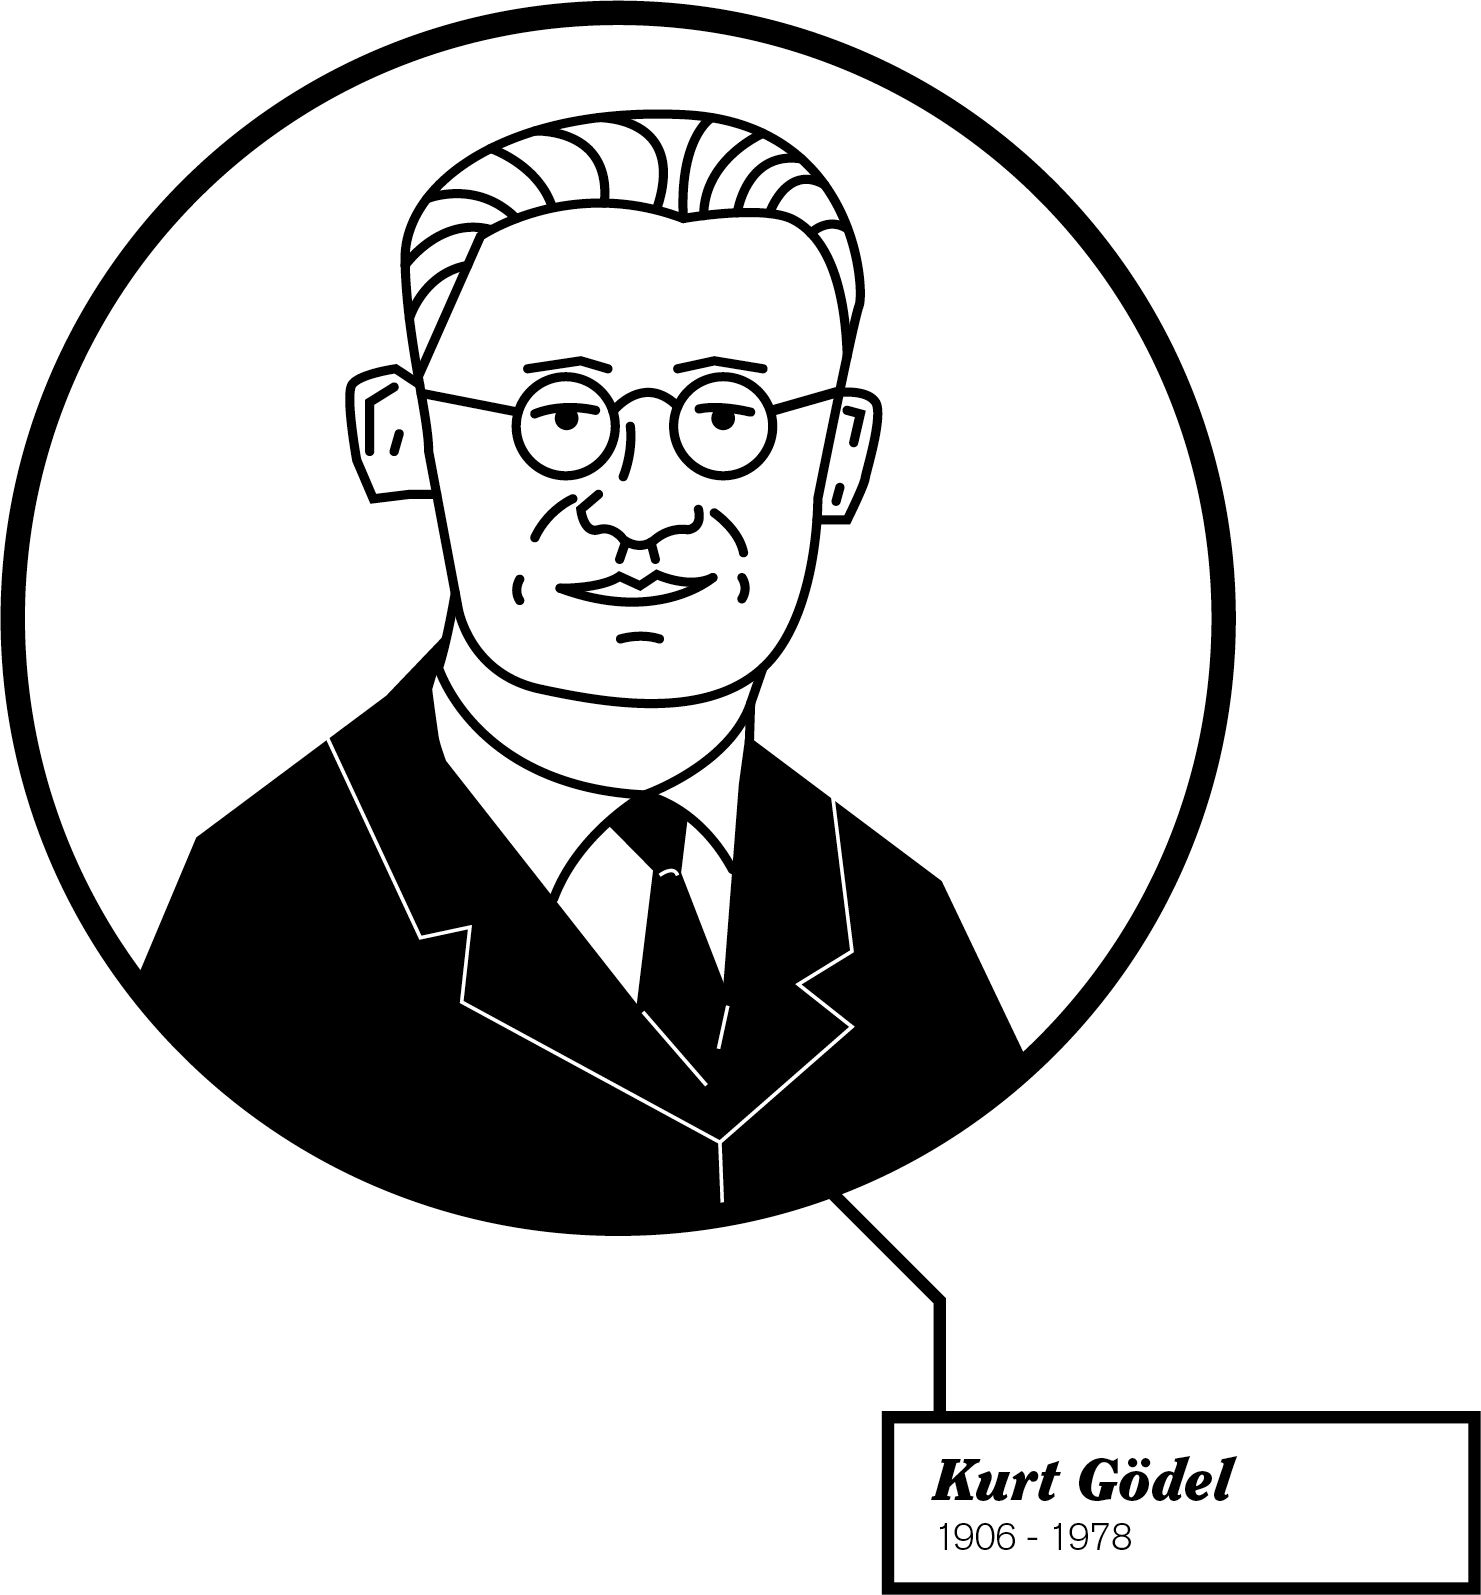
\includegraphics[width=\textwidth]{illustrations/GodelChapter}
\vfill

\olimport*[first-order-logic]{first-order-logic}

\cleartoverso
\ifodd\value{page}\stepcounter{page}\fi
\thispagestyle{empty}
\ \vfill
\noindent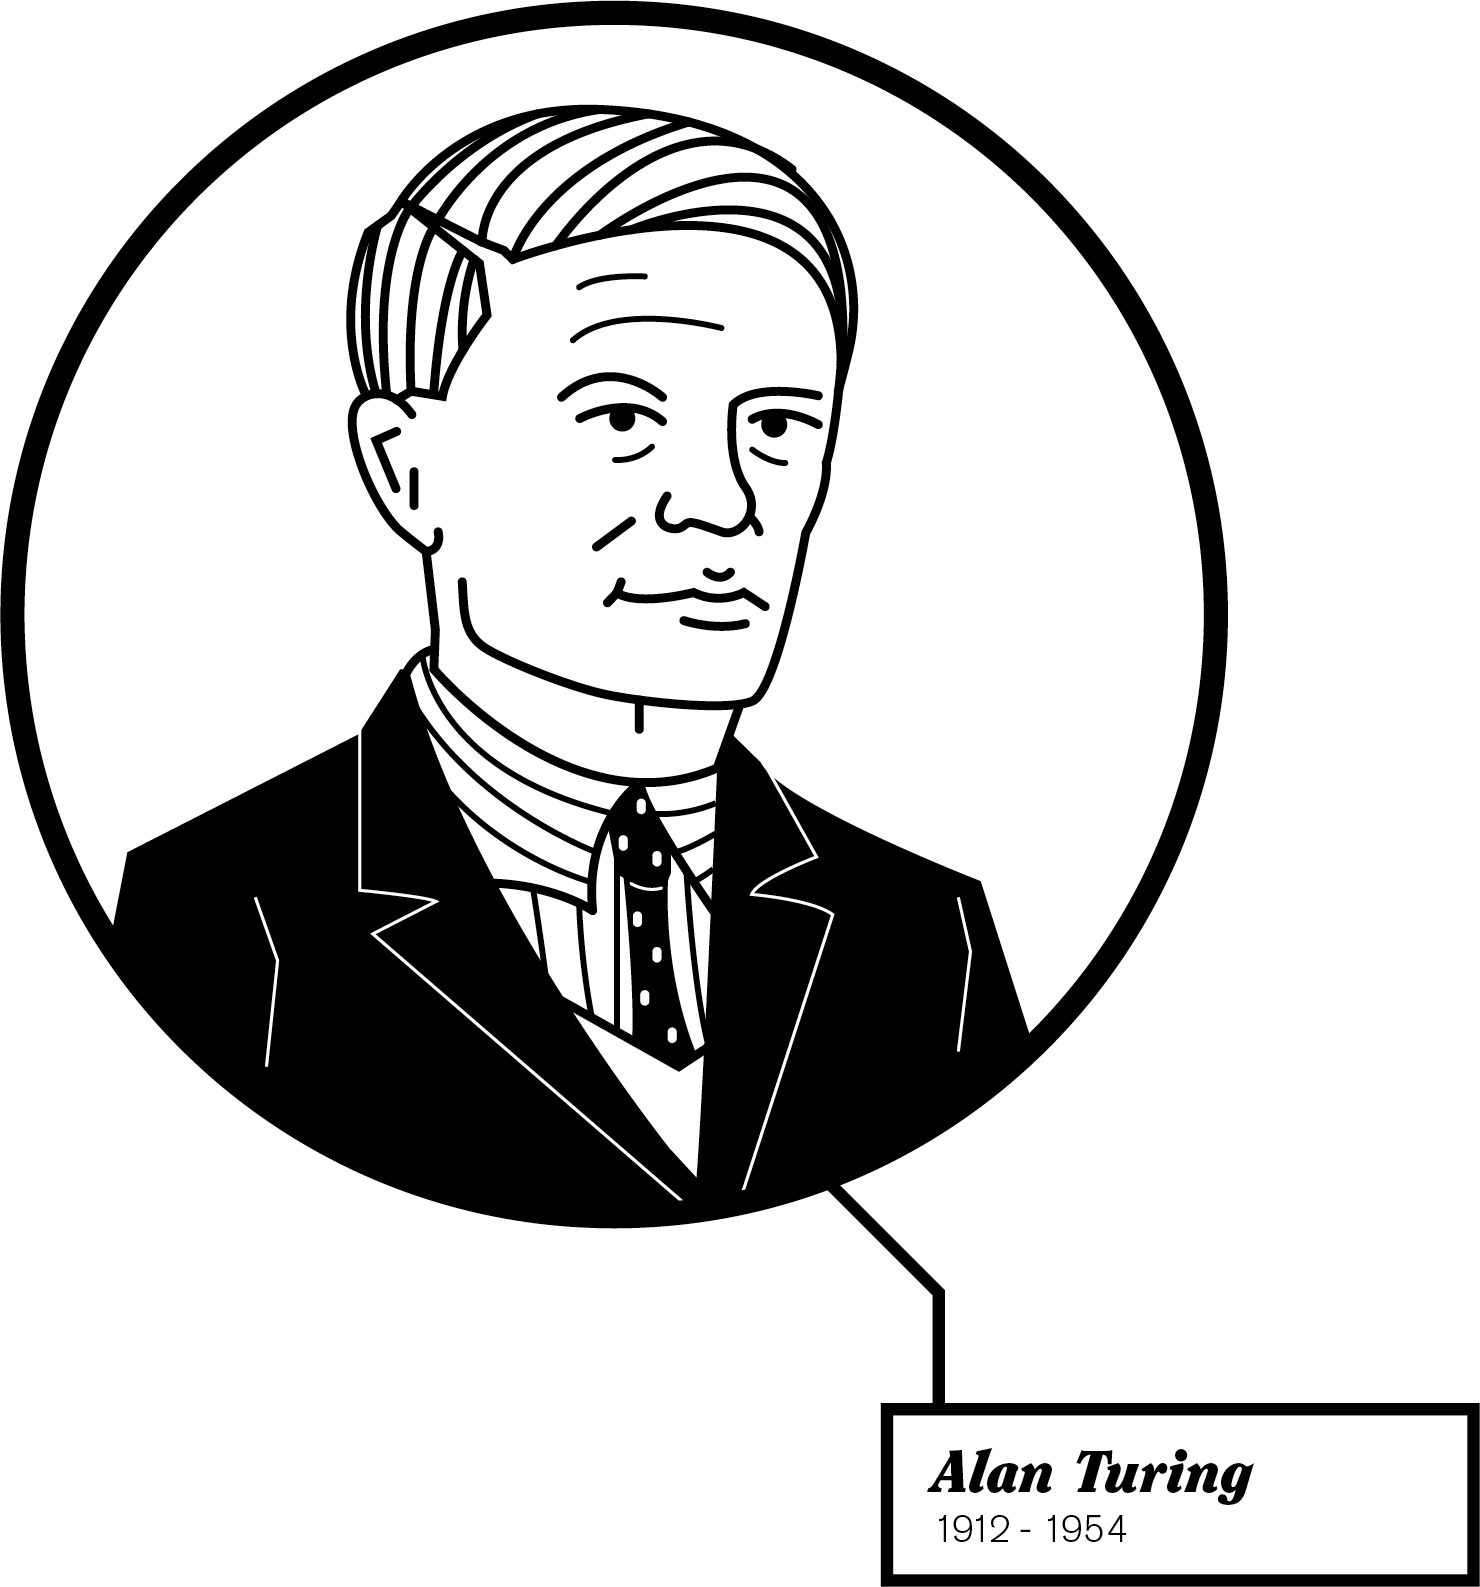
\includegraphics[width=\textwidth]{illustrations/TuringChapter}
\vfill

\olimport*[turing-machines]{turing-machines}

% appendices

\cleartoverso
\ifodd\value{page}\stepcounter{page}\fi
\thispagestyle{empty}
\ \vfill
\noindent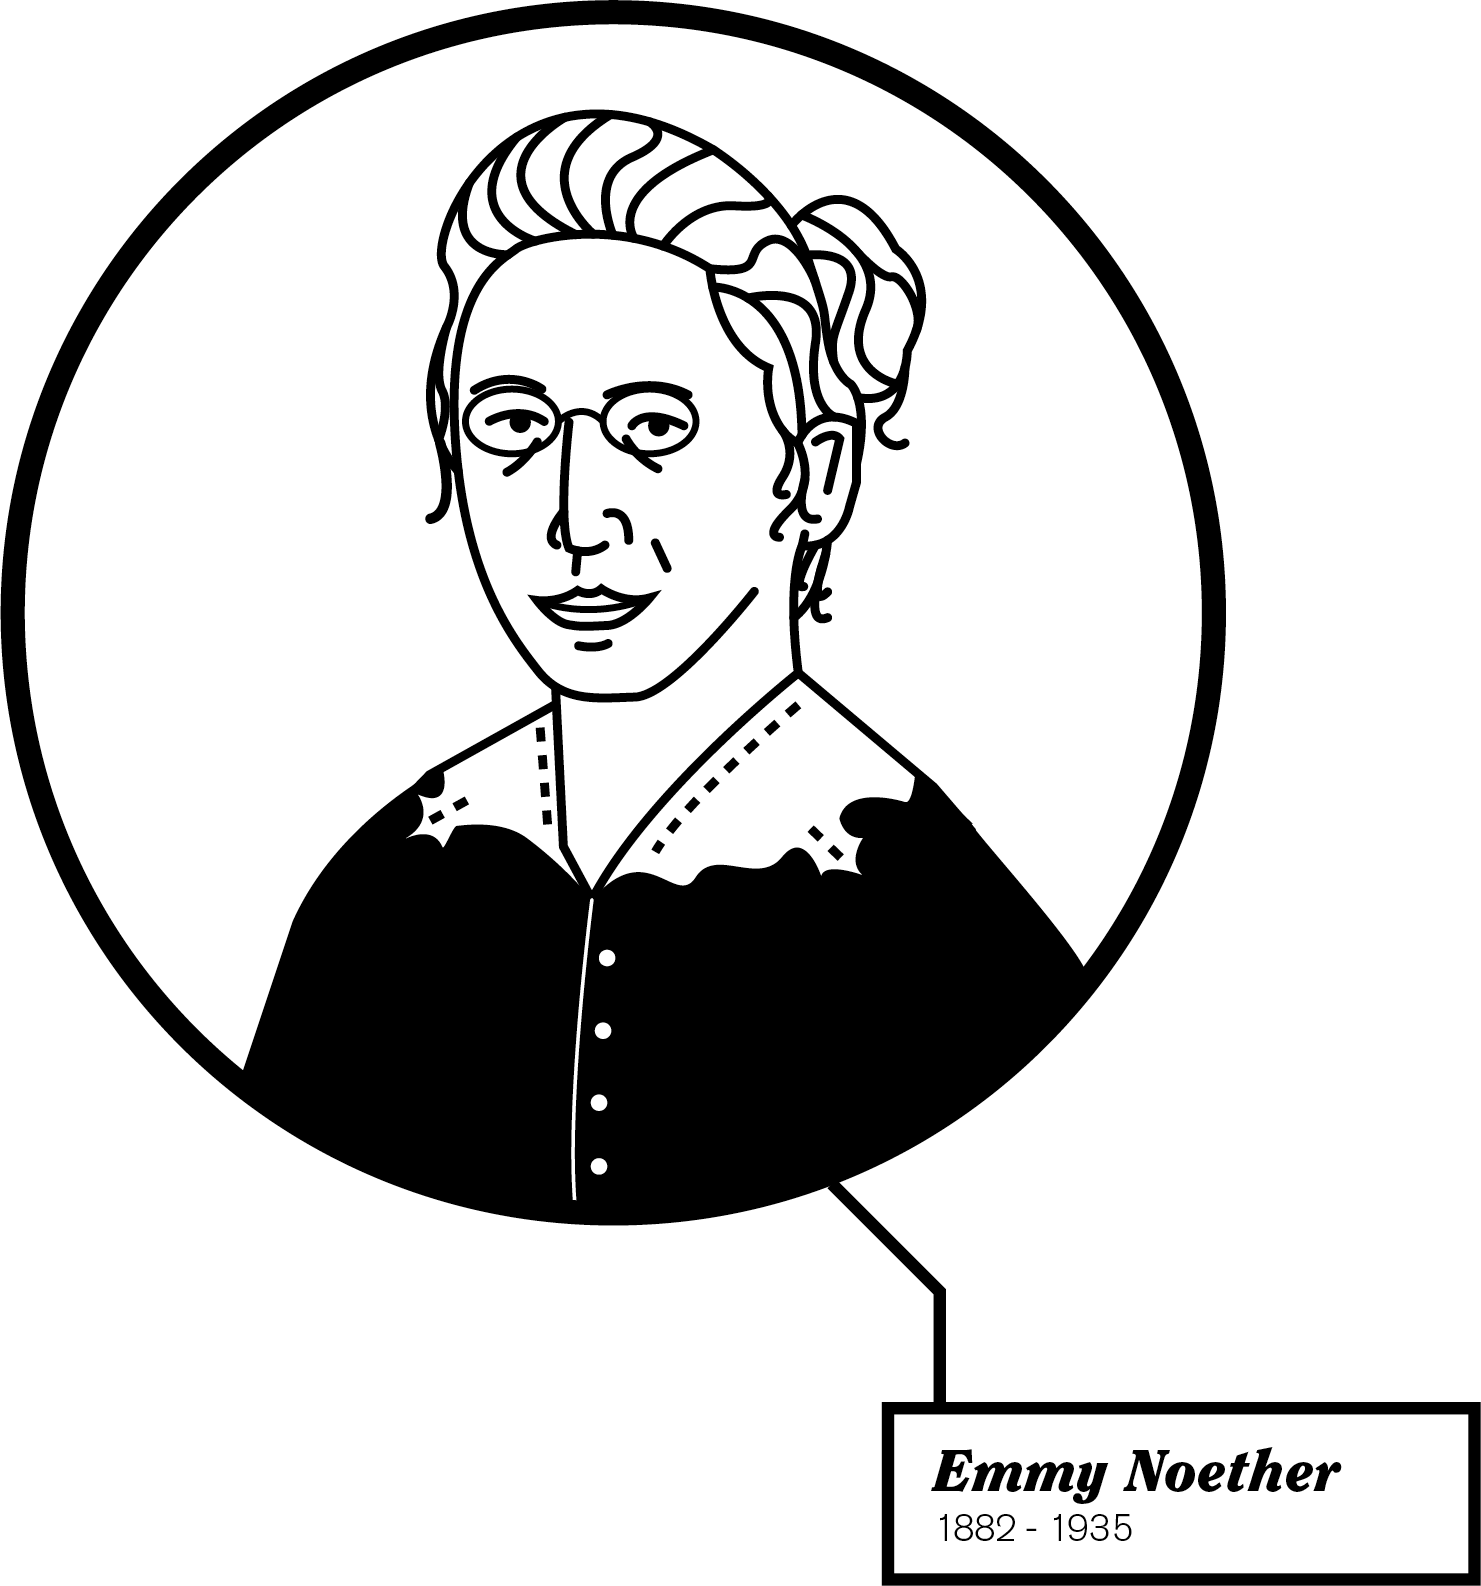
\includegraphics[width=\textwidth]{illustrations/NoetherChapter}
\vfill

\slcChapterSummariesfalse
\appendix

\olimport*[methods/proofs]{proofs}

\olimport*[methods/induction]{induction}

\stopproblems
\def\ifproblems#1{}

\setlength{\olphotowidth}{.45\textwidth}

\chapter{चरित्रे}

\olimport*[history/biographies]{georg-cantor}

\olimport*[history/biographies]{alonzo-church}

\olimport*[history/biographies]{gerhard-gentzen}

\olimport*[history/biographies]{kurt-goedel}

\olimport*[history/biographies]{emmy-noether}

\olimport*[history/biographies]{bertrand-russell}

\olimport*[history/biographies]{alfred-tarski}

\olimport*[history/biographies]{alan-turing}

\olimport*[history/biographies]{ernst-zermelo}

\olimport*[reference/greek-alphabet]{greek-alphabet}

%\backmatter

\glsaddall
\printglossary[style=index,title=शब्दसूची,toctitle=शब्दसूची]

\clearpage
\photocredits

\bibliographystyle{natbib-oup}
\bibliography{\olpath/bib/open-logic}

{% The two-line Marathi heading leaves less room for the About text.
\addtolength{\beforechapskip}{-\baselineskip}%
\addtolength{\afterchapskip}{-\baselineskip}%
\AddToHookNext{cmd/memchapstarinfo/after}{\markboth{ओपन लॉजिक प्रकल्पाविषयी}{ओपन लॉजिक प्रकल्पाविषयी}}%
\olimport*{\olpath/locale/\ollangid/content/open-logic-about}\par}


\end{document}